% This is samplepaper.tex, a sample chapter demonstrating the
% LLNCS macro package for Springer Computer Science proceedings;
% Version 2.20 of 2017/10/04
%
\documentclass[runningheads]{llncs}
%
\usepackage[colorlinks=true,allcolors=blue]{hyperref}
\usepackage{amsmath,amssymb,amsfonts}
\renewcommand\UrlFont{\color{blue}\rmfamily}
\usepackage{multirow}
\usepackage{booktabs}
\usepackage{placeins}
\usepackage{bm}
\usepackage{subfigure} 
\usepackage{floatrow}
\newfloatcommand{capbtabbox}{table}[][\FBwidth]
\floatsetup[table]{capposition=top}
%
\usepackage{graphicx}
\usepackage{longtable}
% Used for displaying a sample figure. If possible, figure files should
% be included in EPS format.
%
% If you use the hyperref package, please uncomment the following line
% to display URLs in blue roman font according to Springer's eBook style:
\renewcommand\UrlFont{\color{blue}\rmfamily}


\begin{document}

\title{Zero-shot Nuclei Detection via Visual-Language Pre-trained Models \textemdash Supplement}
%
%\titlerunning{Abbreviated paper title}
% If the paper title is too long for the running head, you can set
% an abbreviated paper title here
%
% \author{First Author\inst{1}\orcidID{0000-1111-2222-3333} \and
% Second Author\inst{2,3}\orcidID{1111-2222-3333-4444} \and
% Third Author\inst{3}\orcidID{2222--3333-4444-5555}}
% \author{Anonymous}
%
% \authorrunning{F. Author et al.}
% \authorrunning{Anonymous}
% First names are abbreviated in the running head.
% If there are more than two authors, 'et al.' is used.
%
% \institute{Princeton University, Princeton NJ 08544, USA \and
% Springer Heidelberg, Tiergartenstr. 17, 69121 Heidelberg, Germany
% \email{lncs@springer.com}\\
% \url{http://www.springer.com/gp/computer-science/lncs} \and
% ABC Institute, Rupert-Karls-University Heidelberg, Heidelberg, Germany\\
% \email{\{abc,lncs\}@uni-heidelberg.de}}
% \institute{Anonymous Organizations \email{***@******.***}}
%
% \maketitle              % typeset the header of the contribution
%
% \begin{abstract}
% Large-scale visual-language pre-trained models (VLPM) have proven their excellent performance in downstream object detection for natural scenes. However, zero-shot nuclei detection on H\&E images via VLPMs remains underexplored. The large gap between medical images and the web-originated text-image pairs used for pre-training makes it a challenging task. In this paper, we attempt to explore the potential of the object-level VLPM, GLIP, for zero-shot nuclei detection. Concretely, an automatic prompts design pipeline is devised based on the association binding trait of VLPM and the image-to-text VLPM BLIP, avoiding empirical manual prompts engineering. We further establish a self-training framework, using the automatically designed prompts to generate the preliminary results as pseudo labels from GLIP and refine the predicted boxes in an iterative manner. Our method achieves a remarkable performance for label-free nuclei detection, surpassing other comparison methods. Foremost, our work demonstrates that the VLPM pre-trained on natural image-text pairs exhibits astonishing potential for downstream tasks in the medical field as well. Code will be released at ****************.***.

% \keywords{ Nuclei Detection \and Unsupervised Learning \and Visual-Language Pre-trained Models \and Prompt Designing \and Zero-shot Learning.}
% \end{abstract}
%
%Compared to natural images, the high density and specialized morphology of nuclei in H\&E stained images pose substantial difficulties for annotation, requiring specialized knowledge and more annotation efforts. This results in an annotation process that is time-consuming, costly, and prone to errors.
%
\section*{Supplement}
\begin{table}[h]
\caption{Effectiveness of self-training strategy. T refers to the teacher and S refers to the students. The results shown here are calculated on the testing set, while the pseudo labels are generated from the training set. The precision and recall are calculated using a threshold IoU of 0.5. The best results are marked in bold. The initial boxes precision obtained by GLIP is relatively high, but there is still a lot of room for improvement in recall. Through self-training, the overall performance continually improved until convergence.}
\begin{center}
\begin{tabular}{c|cccccc}
\hline
\textbf{Teacher/Students} & \textbf{Precision} & \textbf{Recall} & \textbf{mAP} & \textbf{AP50} & \textbf{AP75} & \textbf{AR} \\ \hline
\textbf{Raw GLIP T0} & 0.678          & 0.310          & 0.146          & 0.252          & 0.165          & 0.213          \\
\textbf{YOLOX S1}    & 0.733          & 0.706         & 0.293          & 0.636          & 0.224          & 0.397          \\
\textbf{YOLOX S2}    & 0.807          & 0.754         & 0.359          & 0.698          & 0.335          & 0.445          \\
\textbf{YOLOX S3}    & \textbf{0.814} & 0.815         & 0.404          & 0.755          & 0.395          & 0.497          \\
\textbf{YOLOX S4}    & 0.813          & \textbf{0.820} & \textbf{0.416} & \textbf{0.808} & 0.382          & 0.502          \\
\textbf{YOLOX S5}    & \textbf{0.814} & 0.807         & 0.414          & 0.742          & \textbf{0.436} & \textbf{0.509} \\ \hline
\end{tabular}
\vskip -0.45in
\label{tab：self}
\end{center}
\end{table}
\begin{table}[h]
\caption{Illustration of the significance of the automatic prompt design using VLPMs for pseudo label generation. Another commonly used unsupervised detection method, superpixels (\textit{Achanta, Radhakrishna, et al. SLIC superpixels compared to state-of-the-art superpixel methods[J]//IEEE TPAMI 2012}), is used to generate pseudo labels in a zero-shot manner. These pseudo labels were then fed into the self-training framework based on the YOLOX segmentation architecture, keeping the settings consistent with using VLPMs for pseudo label generation. The results reveal poor performance.}
\begin{center}
\begin{tabular}{c|cccc}
\hline
\textbf{Teacher/Students} & \textbf{mAP} & \textbf{AP50} & \textbf{AP75} & \textbf{AR} \\ \hline
\textbf{Superpixels T0} & 0.027 & 0.075 & 0.012 & 0.035 \\
\textbf{YOLOX s1} & 0.260 & 0.612 & 0.162 & 0.373 \\
\textbf{YOLOX s2} & 0.272 & 0.617 & 0.183 & 0.392 \\
\textbf{YOLOX s3} & \textbf{0.284} & \textbf{0.655} & 0.169 & \textbf{0.404} \\
\textbf{YOLOX s4} & 0.279 & 0.614 & \textbf{0.213} & 0.389 \\ \hline
\end{tabular}
\vskip -0.45in
\label{tab：superpixel}
\end{center}
\end{table}
\begin{table}[h]
\caption{Results of using DETR (\textit{Carion, Nicolas, et al. End-to-end object detection with transformers[C]//Computer Vision–ECCV 2020}) instead of YOLOX as the detection architecture for self-training in our method.}
\begin{center}
\begin{tabular}{c|cccc}
\hline
\textbf{method} & \textbf{mAP} & \textbf{AP50} & \textbf{AP75} & \textbf{AR} \\ \hline
\textbf{fully-supervised DETR} & 0.404 & 0.749 & 0.398 & 0.501 \\
\textbf{Ours+DETR} & 0.388 & 0.731 & 0.376 & 0.487 \\ \hline
\end{tabular}
\vskip -0.45in
\label{tab：detr}
\end{center}
\end{table}

\begin{figure}[h]
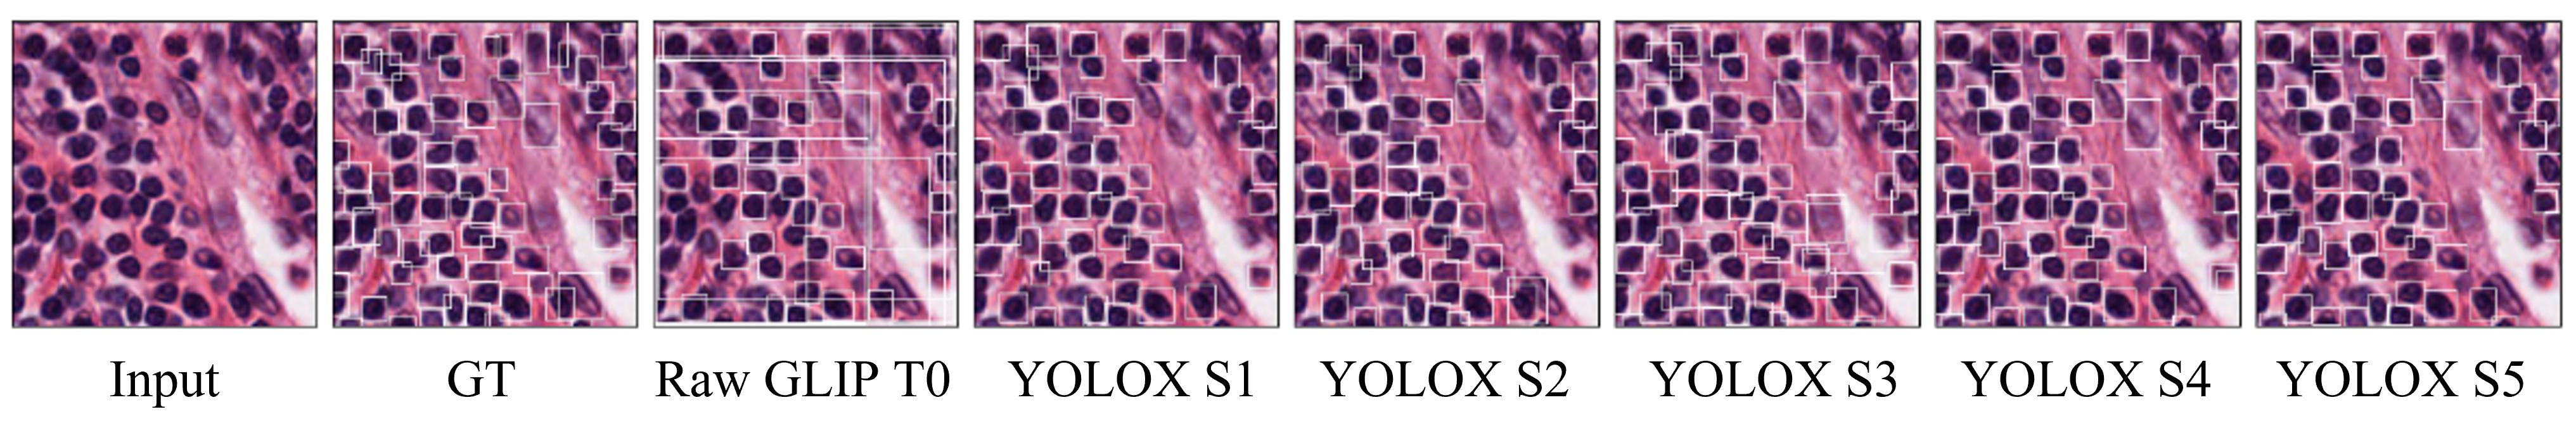
\includegraphics[width=\textwidth]{self-training.png}
\caption{Output visualizations of different stages in the self-training process. From left to right: input image, the ground truth, raw GLIP teacher, YOLOX students.} \label{fig2}
\end{figure}
\begin{figure}[h]
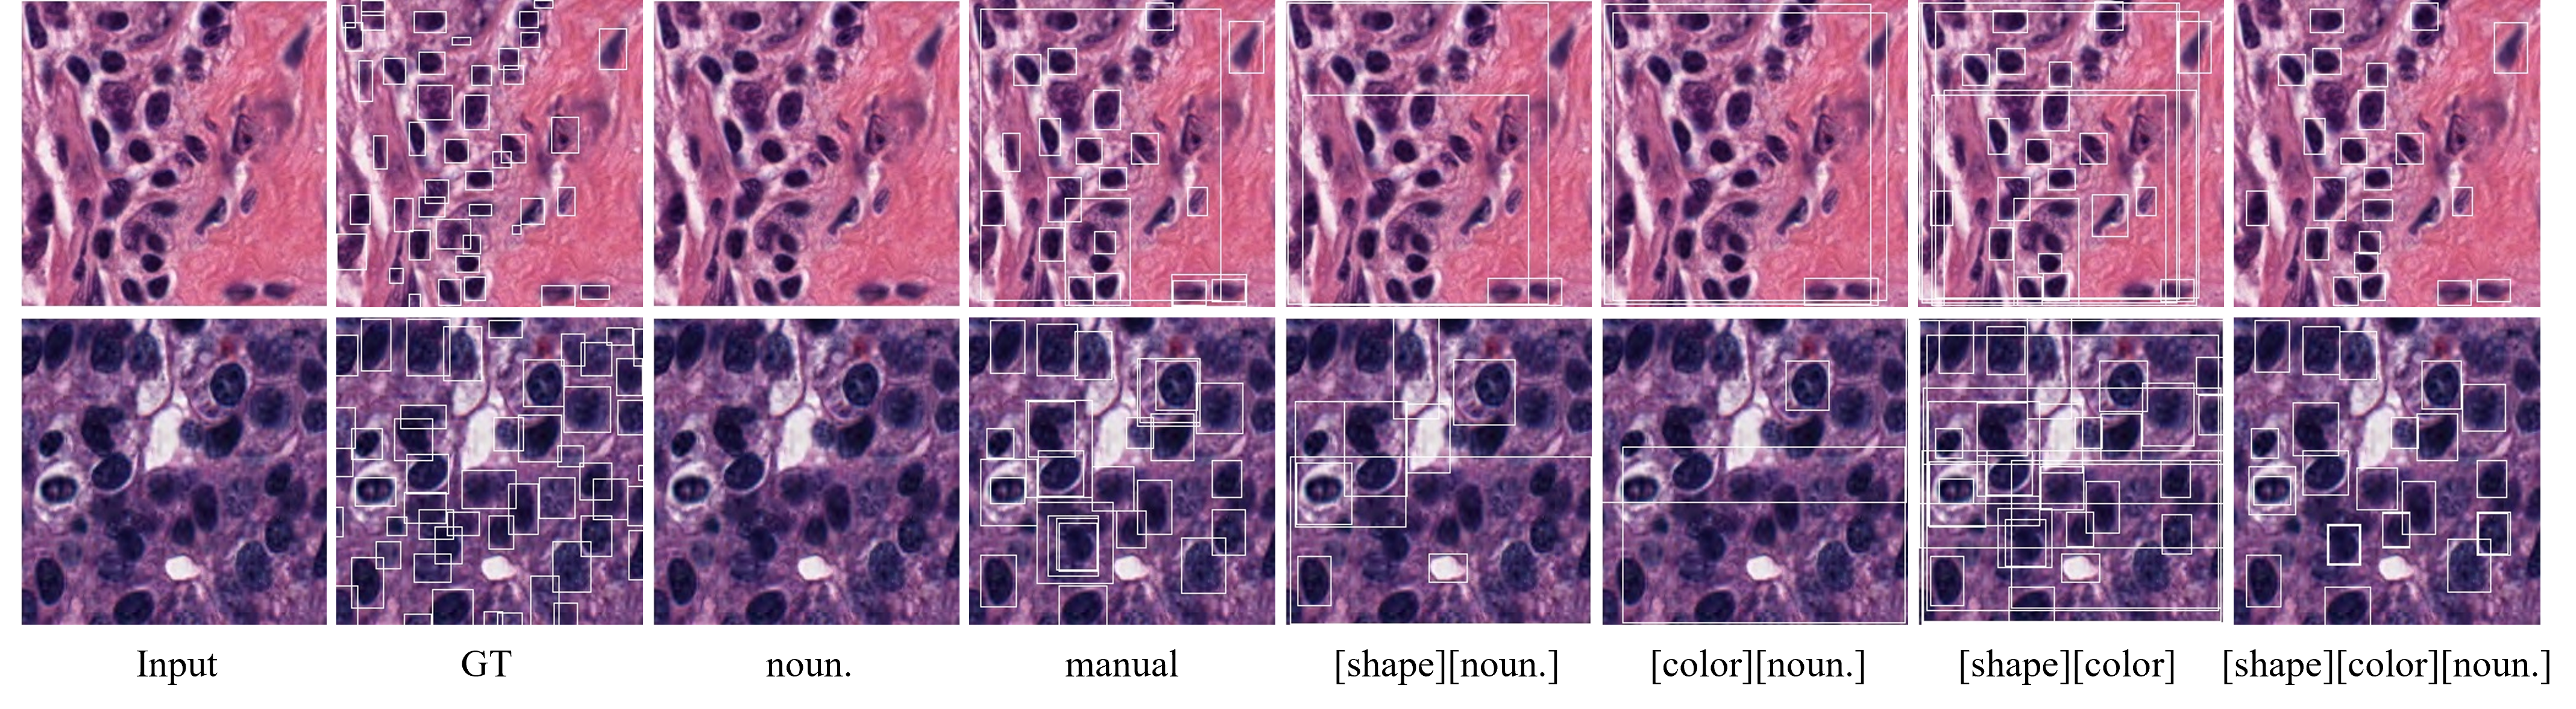
\includegraphics[width=\textwidth]{promptVis.png}
\caption{GLIP prediction visualizations of adopting different prompt design methods. From left to right: input image, the ground truth, different prompt design methods corresponding to Table 2 of the main text.} \label{figprompt}
\end{figure}
\begin{table}[t]
\caption{Detailed list of [shape] and [color]. The first row contains the 3 most frequent words generated by BLIP. The second row shows the synonyms augmented by GPT.}
\begin{center}
\resizebox{\textwidth}{!}{
\begin{tabular}{c|c|c}
\hline
\textbf{}          & \textbf{{[}shape{]}}                       & \textbf{{[}color{]}}                            \\ \hline
\textbf{From BLIP} & round, circle, oblong                      & blue, black, purple                               \\ \hline
\multirow{3}{*}{\textbf{Synonyms}} & oval, elliptical, rectangular, Oblate, & magenta, deep purple, dark purple, lilac, \\
                   & rectilinear, circular, ring, disc, loop, cycle, & violet, azure, aqua, cyan, light blue, turquoise, \\
                   & spherical, curved, rounded, cyclical & light blue, sky blue, ebony, coal, jet, pitch, onyx \\ \hline
\end{tabular}%
}
\label{tab：words}
\end{center}
\end{table}
\begin{table}[t]
\caption{Comparison with CLIP-based zero-shot object detection methods, VL-PLM (\textit{Zhao S, Zhang Z, Schulter S, et al. Exploiting unlabeled data with vision and language models for object detection[C]//Computer Vision–ECCV 2022}) and VLDet (\textit{Lin C, Sun P, Jiang Y, et al. Learning Object-Language Alignments for Open-Vocabulary Object Detection[C]//ICLR 2023}). Our method is GLIP-based. The results demonstrate the superiority of GLIP over CLIP in zero-shot transfer to nuclei detection.}
\centering
% \resizebox{\columnwidth}{!}{%
\begin{tabular}{c|cccc}
\hline
\textbf{method}        & \textbf{mAP}   & \textbf{AP50}  & \textbf{AP75}  & \textbf{AR}    \\ \hline
\textbf{VL-PLM (2022)} & 0.333          & 0.582          & 0.342          & 0.501          \\
\textbf{VLDet (2023)}  & 0.173          & 0.407          & 0.112          & 0.263          \\ \hline
\textbf{Ours}          & \textbf{0.416} & \textbf{0.808} & \textbf{0.382} & \textbf{0.502} \\ \hline
\end{tabular}%
% }
\end{table}
% \qquad
% \newpage
% \begin{center}
% \begin{longtable}{p{3cm}|p{4cm}|p{4cm}}
% \caption{Detailed list of [shape] and [color]. The first row contains the top 3 frequent words generated by BLIP. The second row shows the synonyms augmented by GPT.}
% \label{tab：component}\\
% \hline
% \textbf{} &
%   \textbf{{[}shape{]}} &
%   \textbf{{[}color{]}} \\ \hline
% \textbf{From BLIP} &
%   round, circle, oblong &
%   blue, black, purple \\ \hline
% \textbf{Synonyms from language model} &
%   oval, elliptical, rectangular, Oblate, rectilinear, circular, ring, disc, loop, cycle, spherical, curved, rounded, cyclincal &
%   magenta, deep purple, dark purple, lilac, violet, azure, aqua, cyan, light blue, turquoise, light blue, sky blue, ebony, coal, jet, pitch, onyx \\ \hline
% \end{longtable}
% \end{center}


% \begin{figure}[t]
% 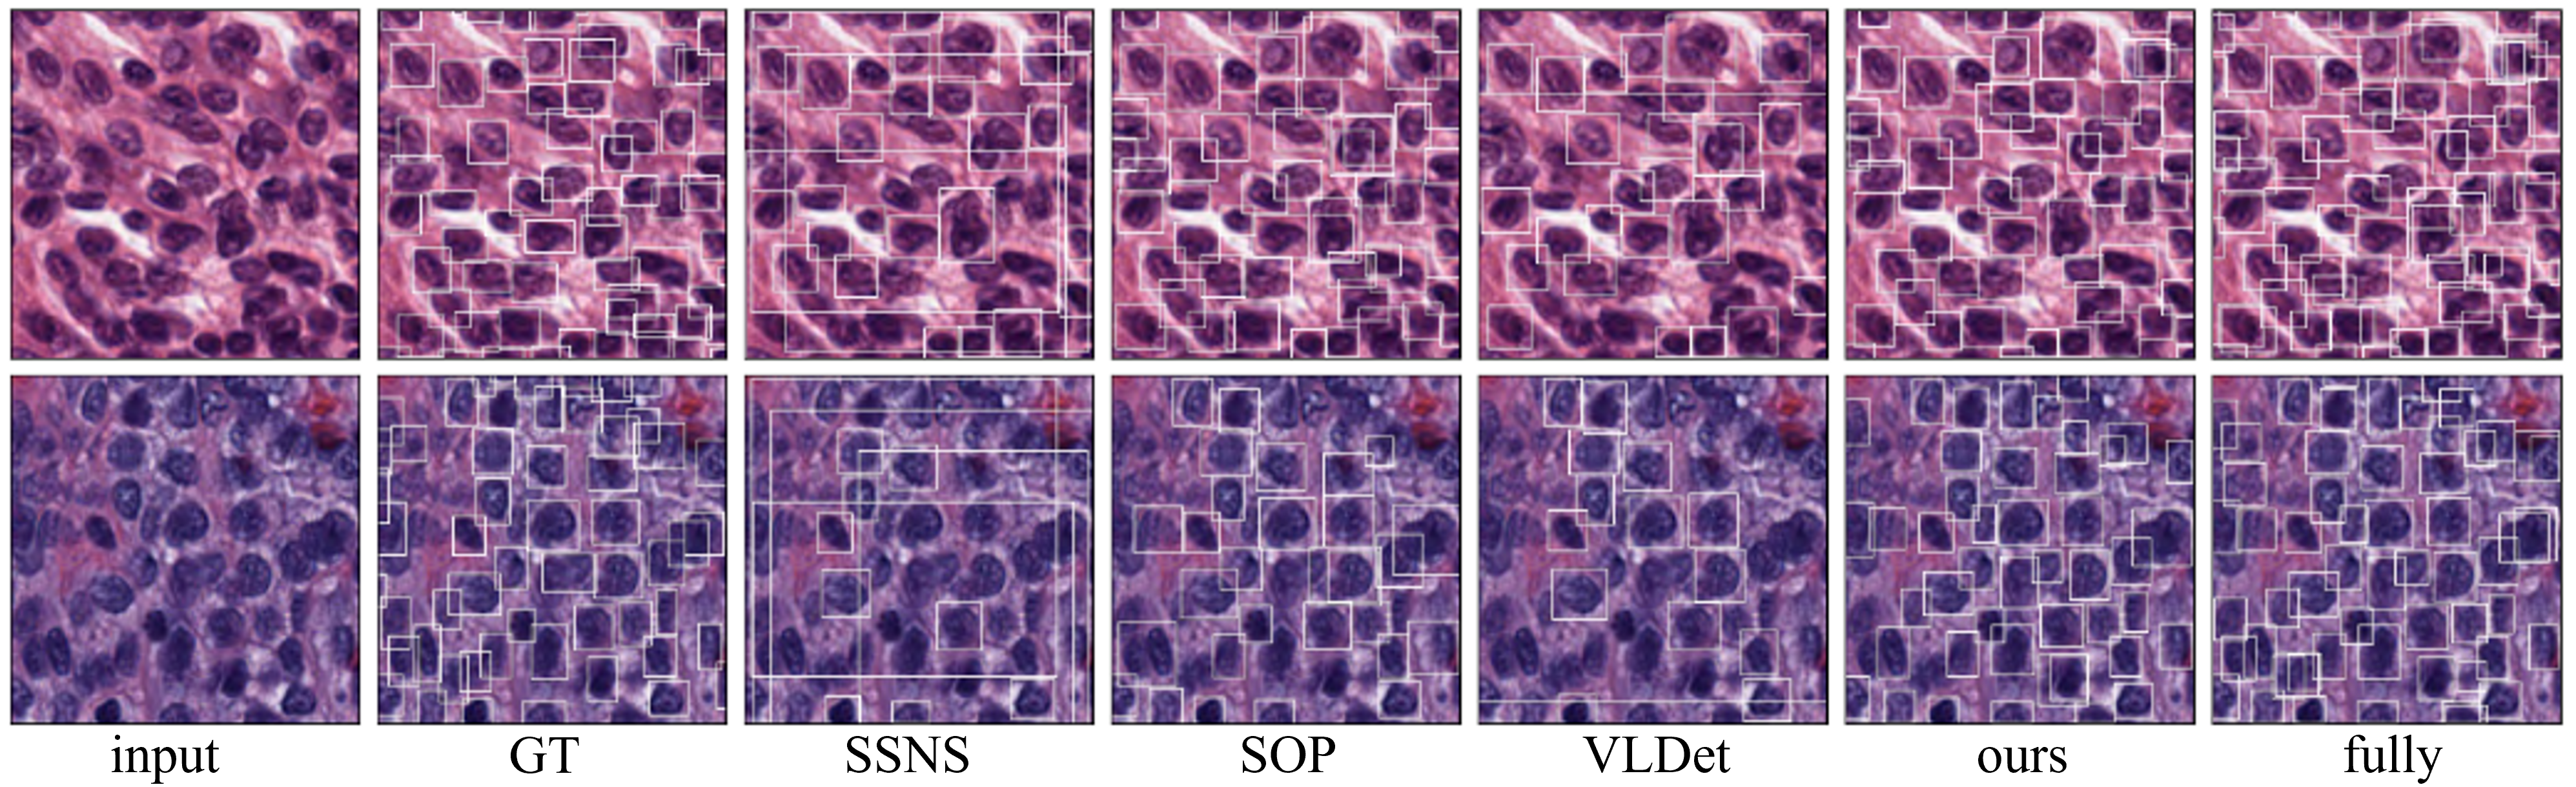
\includegraphics[width=\textwidth]{comparison.png}
% \caption{Output visualizations of different stages in self-training process. From left to right: raw GLIP teacher, YOLOX students.} \label{fig2}
% \end{figure}

% \begin{table}[t]
% \caption{Ablation study of prompt components. ``\'': no attribute words, ``WO A Aug.'': only with attribute words generated by BLIP, ``W A Aug.'': with attribute augmentation, ``WO N Aug.'': noun list only contains ``nuclei'', ``W N Aug.'': with noun augmentation. Applying noun augmentation leads to suboptimum results because augmented new synonym nouns are uncommon and may not appear in the pre-training data that GLIP used. However, applying attribute word augmentation is generally effective because augmented attribute words are also common descriptions for natural scenes.}
% \begin{center}
% \begin{tabular}{c|c|cccc}
% \hline
% \textbf{attribute}                         & \textbf{Noun}      & \textbf{mAP} & \textbf{AP50} & \textbf{AP75} & \textbf{AR} \\ \hline
% \multirow{2}{*}{\textbf{\textbackslash{}}} & \textbf{WO N Aug.} & 0.080        & 0.161         & 0.070         & 0.239       \\
%                                            & \textbf{W N Aug.}  & 0.064        & 0.152         & 0.036         & 0.150       \\ \hline
% \multirow{2}{*}{\textbf{WO A Aug.}}        & \textbf{WO N Aug.} & 0.372        & 0.725         & 0.337         & 0.464       \\
%                                            & \textbf{W N Aug.}  & 0.316        & 0.754         & 0.182         & 0.419       \\ \hline
% \multirow{2}{*}{\textbf{W A Aug.}} & \textbf{WO N Aug.} & \textbf{0.416} & \textbf{0.808} & \textbf{0.382} & \textbf{0.502} \\
%                                            & \textbf{W N Aug.}  & 0.332        & 0.659         & 0.296         & 0.434       \\ \hline
% \end{tabular}
% \label{tab：component}
% \end{center}
% \end{table}


% \begin{table*}[t]
% \begin{floatrow}
% \capbtabbox{ 
% \resizebox{0.45\textwidth}{!}{
% \renewcommand{\arraystretch}{1}
% \begin{tabular}{c|cccc}
% \hline
% \textbf{prompt design} & \textbf{mAP} & \textbf{AP50} & \textbf{AP75} & \textbf{AR} \\ \hline
% \textbf{noun. \cite{li2022grounded}} & 0.064 & 0.152 & 0.036 & 0.150 \\
% \textbf{manual design \cite{li2022grounded}} & 0.414 & 0.757 & 0.422 & 0.509 \\ \hline
% \textbf{auto: {[}shape{]}{[}noun.{]}} & 0.336 & 0.604 & 0.350 & 0.434 \\
% \textbf{auto: {[}color{]}{[}noun.{]}} & 0.213 & 0.447 & 0.176 & 0.325 \\
% \textbf{auto: {[}shape{]}{[}color{]}} & 0.413 & 0.726 & 0.438 & 0.498 \\
% \textbf{auto:{[}shape{]}{[}color{]}{[}noun.{]}} & \textbf{0.416} & \textbf{0.808} & \textbf{0.382} & \textbf{0.502} \\ \hline
% \end{tabular} 
% }
% }{
%  \caption{Results of adopting different prompt design methods. The pompts of last 4 rows are automatically generated. The best results are marked in \textbf{bold}.}
%  \label{tab:prompt}
% }

% \capbtabbox{ 
% \resizebox{0.45\textwidth}{!}{
% \renewcommand{\arraystretch}{1.13}
% \begin{tabular}{c|c|cccc}
% \hline
% \textbf{A Aug.} & \textbf{N Aug.} & \textbf{mAP} & \textbf{AP50} & \textbf{AP75} & \textbf{AR} \\ \hline
%  &  & 0.372 & 0.725 & 0.337 & 0.464 \\
% \checkmark &  & \textbf{0.416} & \textbf{0.808} & \textbf{0.382} & \textbf{0.502} \\
%  & \checkmark & 0.316 & 0.754 & 0.182 & 0.419 \\
% \checkmark & \checkmark & 0.332 & 0.659 & 0.296 & 0.434 \\ \hline
% \end{tabular}
% }
% }{
%  \caption{Ablation study on word augmentation. ``A Aug.'' and ``N Aug.'' refer to attribute augmentation and noun augmentation, respectively.}
%  \label{tab: aug}
% }


% \end{floatrow} 
% \end{table*}




% according to the changes in the corresponding domain

% ---- Bibliography ----
%
% BibTeX users should specify bibliography style 'splncs04'.
% References will then be sorted and formatted in the correct style.
%

% \textcolor{white}{\bibliographystyle{splncs04}}
% \textcolor{white}{\bibliography{mybibliography}}
%
% \begin{thebibliography}{8}
% \bibitem{ref_article1}
% Author, F.: Article title. Journal \textbf{2}(5), 99--110 (2016)

% \bibitem{ref_lncs1}
% Author, F., Author, S.: Title of a proceedings paper. In: Editor,
% F., Editor, S. (eds.) CONFERENCE 2016, LNCS, vol. 9999, pp. 1--13.
% Springer, Heidelberg (2016). \doi{10.10007/1234567890}

% \bibitem{ref_book1}
% Author, F., Author, S., Author, T.: Book title. 2nd edn. Publisher,
% Location (1999)

% \bibitem{ref_proc1}
% Author, A.-B.: Contribution title. In: 9th International Proceedings
% on Proceedings, pp. 1--2. Publisher, Location (2010)

% \bibitem{ref_url1}
% LNCS Homepage, \url{http://www.springer.com/lncs}. Last accessed 4
% Oct 2017
% \end{thebibliography}
\end{document}
